\documentclass[svgnames,
               hyperref={colorlinks,citecolor=DeepPink4,linkcolor=FireBrick,urlcolor=Maroon},
               usepdftitle=false]  % see \hypersetup{} below
               {beamer}

\mode<presentation>{
  \usetheme{Madrid}
  \usecolortheme{seagull}
  \setbeamercovered{transparent}
  \setbeamerfont{frametitle}{size=\large}
}

\setbeamercolor*{block title}{bg=red!10}
\setbeamercolor*{block body}{bg=red!5}

%\usepackage[svgnames]{xcolor}
\usepackage{hyperref}
\hypersetup{
    pdftitle = {Glacial flows, simulated faster},
    pdfauthor = {Ed Bueler},
    pdfsubject = {},
    pdfkeywords = {}
}

\usepackage[english]{babel}
\usepackage[latin1]{inputenc}
\usepackage{times}
\usepackage[T1]{fontenc}
\usepackage{empheq,bm,xspace,fancyvrb,soul}
\usepackage{tikz}
\usetikzlibrary{shapes,arrows.meta,decorations.markings,decorations.pathreplacing,fadings,positioning}
\usepackage[kw]{pseudo}
\pseudoset{left-margin=15mm,topsep=5mm,idfont=\texttt,st-left=,st-right=}

\newcommand{\eps}{\epsilon}
\newcommand{\RR}{\mathbb{R}}

\newcommand{\grad}{\nabla}
\newcommand{\Div}{\nabla\cdot}
\newcommand{\trace}{\operatorname{tr}}

\newcommand{\hbn}{\hat{\mathbf{n}}}

\newcommand{\bb}{\mathbf{b}}
\newcommand{\be}{\mathbf{e}}
\newcommand{\bbf}{\mathbf{f}}
\newcommand{\bg}{\mathbf{g}}
\newcommand{\bn}{\mathbf{n}}
\newcommand{\bq}{\mathbf{q}}
\newcommand{\br}{\mathbf{r}}
\newcommand{\bu}{\mathbf{u}}
\newcommand{\bv}{\mathbf{v}}
\newcommand{\bw}{\mathbf{w}}
\newcommand{\bx}{\mathbf{x}}

\newcommand{\bF}{\mathbf{F}}
\newcommand{\bQ}{\mathbf{Q}}
\newcommand{\bU}{\mathbf{U}}
\newcommand{\bV}{\mathbf{V}}
\newcommand{\bX}{\mathbf{X}}

\newcommand{\btau}{\bm{\tau}}
\newcommand{\bxi}{\bm{\xi}}

\newcommand{\bzero}{\bm{0}}

\newcommand{\rhoi}{\rho_{\text{i}}}

\newcommand{\ip}[2]{\left(#1,#2\right)}

\newcommand{\mR}{R^{\bm{\oplus}}}
\newcommand{\iR}{R^{\bullet}}

\newcommand{\nn}{{\text{n}}}
\newcommand{\pp}{{\text{p}}}
\newcommand{\qq}{{\text{q}}}
\newcommand{\rr}{{\text{r}}}

\newcommand{\bus}{\bu|_s}
\newcommand{\oo}[1]{\displaystyle O\left(#1\right)}
\newcommand{\sold}{s_{\text{o}}}


\title{Glacial flows, simulated faster}

%\subtitle{\emph{x}}

\author{Ed Bueler}

\institute[UAF]{University of Alaska Fairbanks}

\date[]{June 2023}

%\titlegraphic{\begin{picture}(0,0)
%    \put(0,180){\makebox(0,0)[rt]{\includegraphics[width=4cm]{figs/software.png}}}
%  \end{picture}
%}

\titlegraphic{\hfill 
\includegraphics[width=0.15\textwidth]{../images/uafbw.png}}

%% to start section counter at 0 see
%% https://tex.stackexchange.com/questions/170222/change-the-numbering-in-beamers-table-of-content


\begin{document}
\beamertemplatenavigationsymbolsempty

%\begin{frame}
%  \maketitle
%\end{frame}

{
  \usebackgroundtemplate{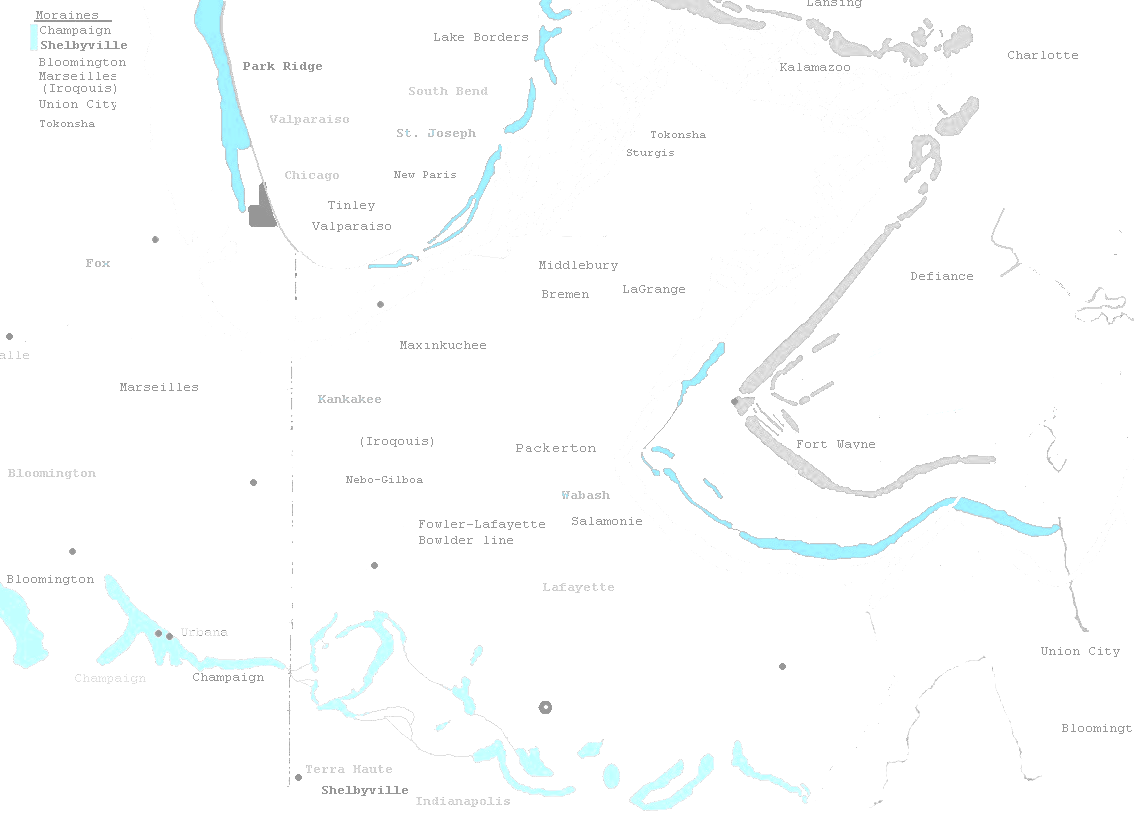
\includegraphics[height=\paperheight]{../images/fade-moraines-indiana.png}}
  \begin{frame}
    \titlepage
  \end{frame}
}

\begin{frame}{Outline}
  \tableofcontents[hideallsubsections]
\end{frame}


\section{introduction to glaciers and ice sheets}

\newcommand{\basicglaciers}[1]{
\begin{frame}{basic facts about glaciers #1}

\begin{columns}
\begin{column}{0.6\textwidth}
\begin{itemize}
\item glacier ice is a \emph{very viscous, incompressible, non-Newtonian fluid}
    \begin{itemize}
    \item[$\circ$] more soon \dots
    \end{itemize}
\item glaciers lie on \emph{topography}
    \begin{itemize}
    \item[$\circ$] except sometimes they float on water (floating tongue or ice shelf)
    \end{itemize}
\item a glacier's geometry (\emph{free surface}), and its velocity, \emph{evolve in contact with the climate}:
    \begin{itemize}
    \item[$\circ$] snowfall
    \item[$\circ$] surface melt
    \item[$\circ$] subglacial melt
    \item[$\circ$] sub-shelf melt (when floating)
    \item[$\circ$] calving (into ocean)
    \end{itemize}
\end{itemize}
\end{column}
\begin{column}{0.42\textwidth}
\hfill 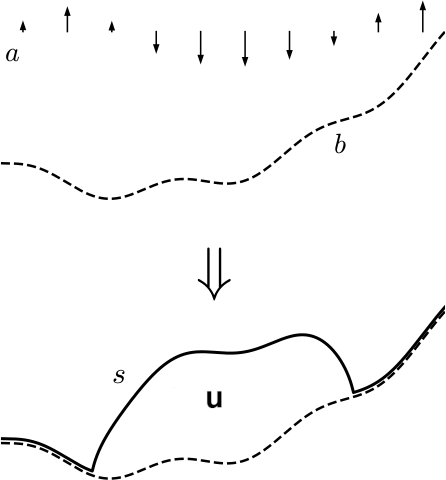
\includegraphics[width=0.9\textwidth]{../images/map-velocity.png}
\end{column}
\end{columns}
\end{frame}
}

\basicglaciers{}

\begin{frame}{pictures of glaciers}

\begin{center}
\only<1>{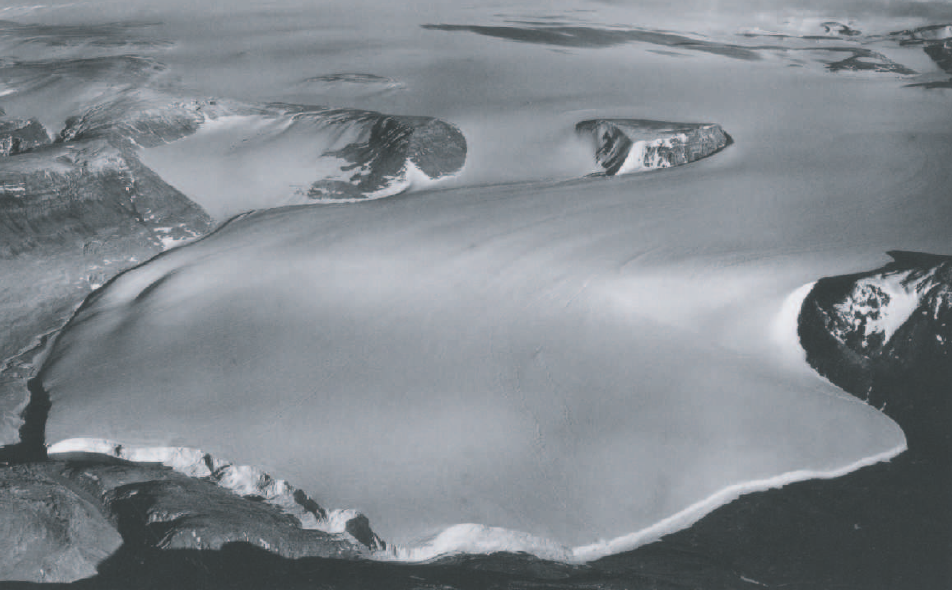
\includegraphics[height=0.8\textheight]{../images/polaris.png}} \only<2>{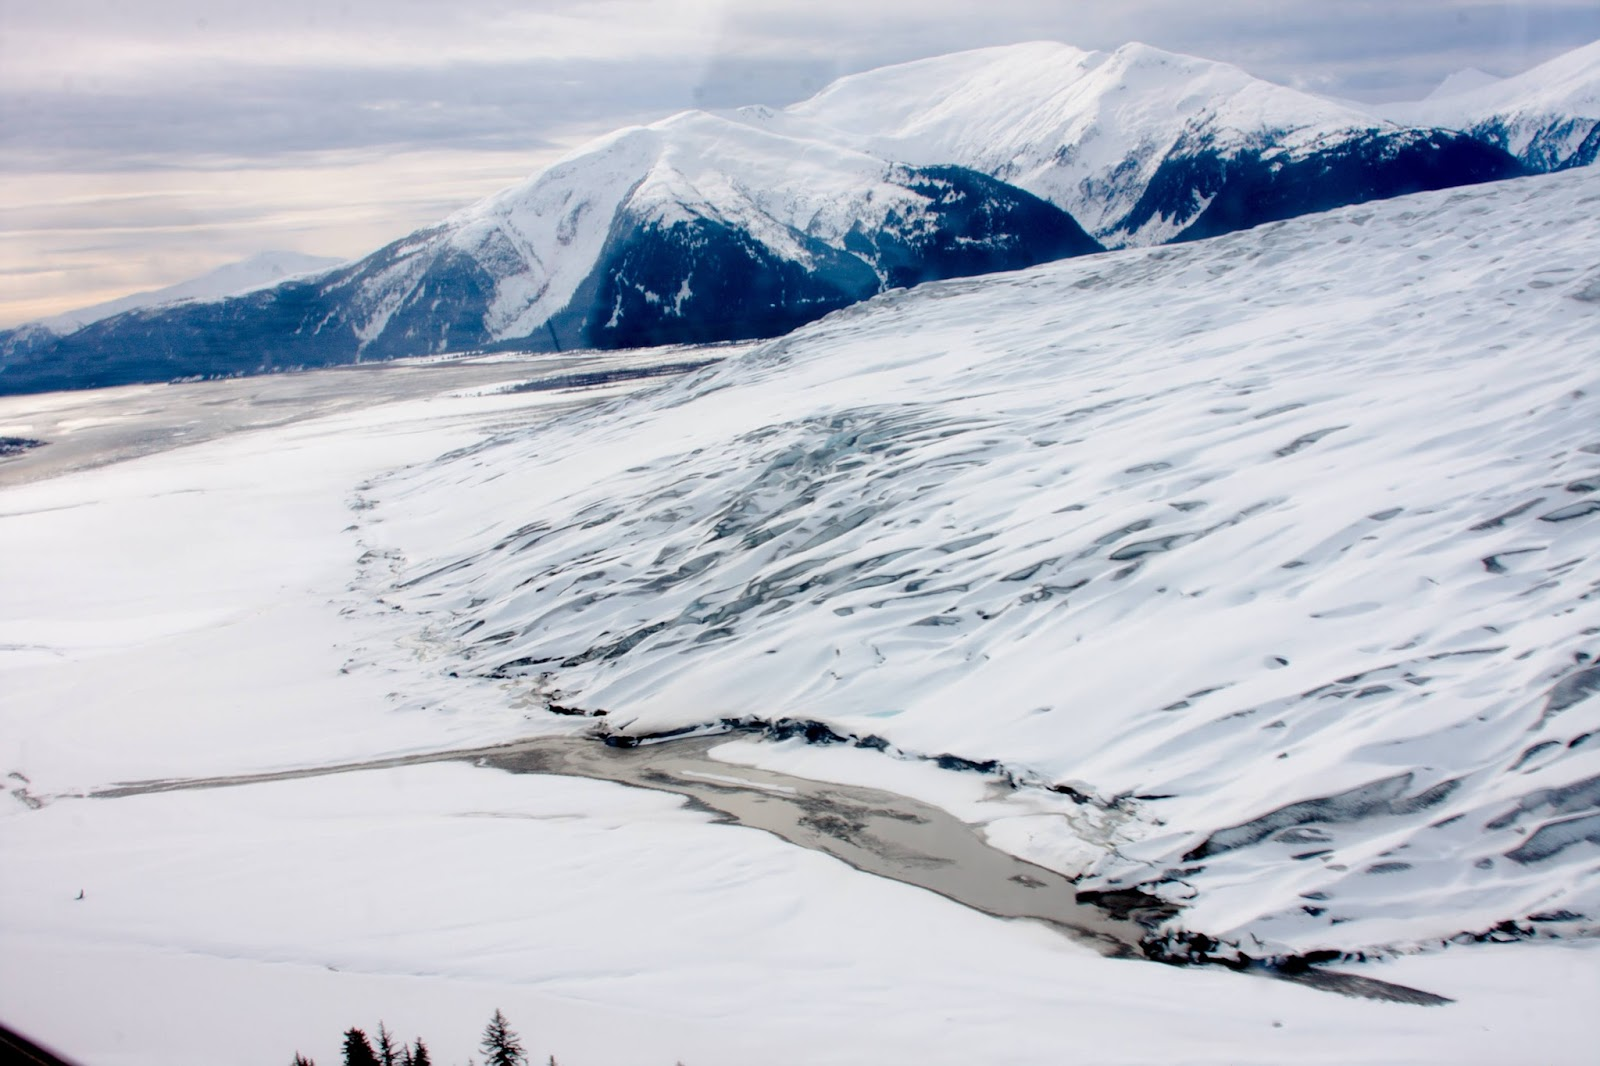
\includegraphics[height=0.8\textheight]{../images/taku-truffer2016.jpg}}
\only<3>{\vspace{-5mm} \mbox{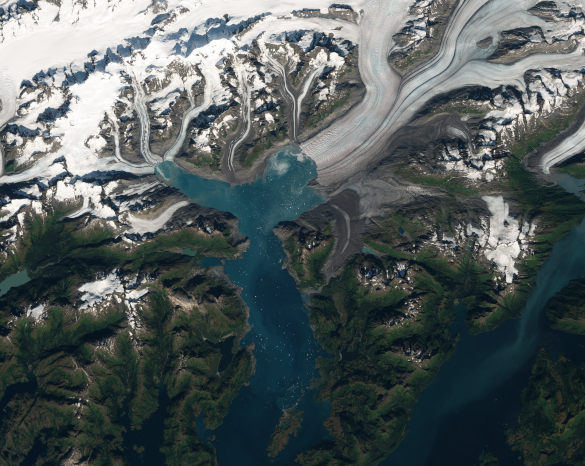
\includegraphics[height=0.8\textheight]{../images/columbiasentinel2.jpg} 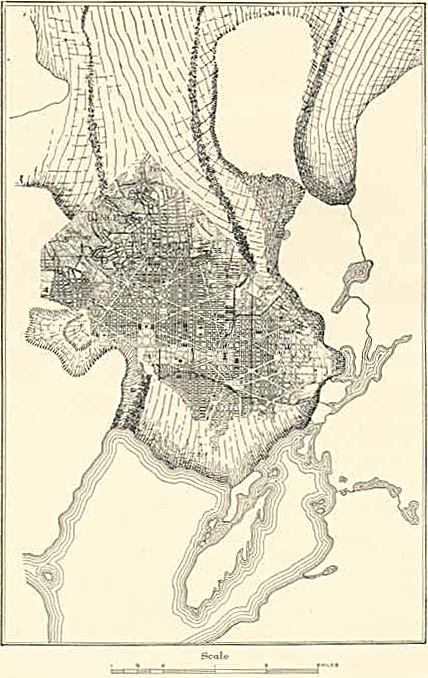
\includegraphics[height=0.55\textheight]{../images/natgeocolumbia1910.png}}}
\end{center}

{\scriptsize
\only<1>{Polaris Glacier \hfill {\tiny (Post and LaChappelle 1971)}}
\only<2>{Taku Glacier \hfill {\tiny (M.~Truffer 2016)}}
\only<3>{Columbia Glacier \hfill {\tiny (Sentinel-2B 2018, National Geographic 1910)}}
}
\end{frame}


\begin{frame}{what is an ice sheet?}

\begin{itemize}
\item \emph{def.} \, \alert{ice sheet} $=$ a large glacier with small thickness$/$width ratio
\end{itemize}

\bigskip
\begin{minipage}[t][60cm][t]{\textwidth}
\begin{center}
\includegraphics<1>[height=0.69\textheight]{../images/ant-pittard2021.png}
\only<1>{\par {\scriptsize Antarctic ice sheet} \hfill {\tiny (Pittard et al 2021)}}
\only<2>{\vspace{17mm}}
\includegraphics<2>[width=\textwidth]{../images/ant-schoofhewitt2013.png}
\only<2>{\vspace{4mm}\par {\scriptsize note smooth surface and rough bed \dots and vertical exaggeration} \hfill {\tiny (Schoof \& Hewitt 2013)}}
\includegraphics<3>[height=0.69\textheight]{../images/alps-seguinot2018.png}
\only<3>{\par {\scriptsize modeled Alpine ice sheet near last glacial maximum} \hfill {\tiny (Seguinot et al 2018)}}
\includegraphics<4>[height=0.69\textheight]{../images/laurentide-margold2018.png}
\only<4>{\par {\scriptsize Laurentide ice sheet, $\approx$ 22,000 years ago} \hfill {\tiny (Margold, Stokes, Clark 2018)}}
\includegraphics<5>[height=0.69\textheight]{../images/moraines-indiana.jpg}
\only<5>{\par {\scriptsize moraines in Illinois, Indiana, Ohio} \hfill {\tiny (Larsen 1986 and other sources)}}
\end{center}
\end{minipage}
\end{frame}


\begin{frame}{finally, an ice sheet is \emph{not} sea ice!}
\begin{center}
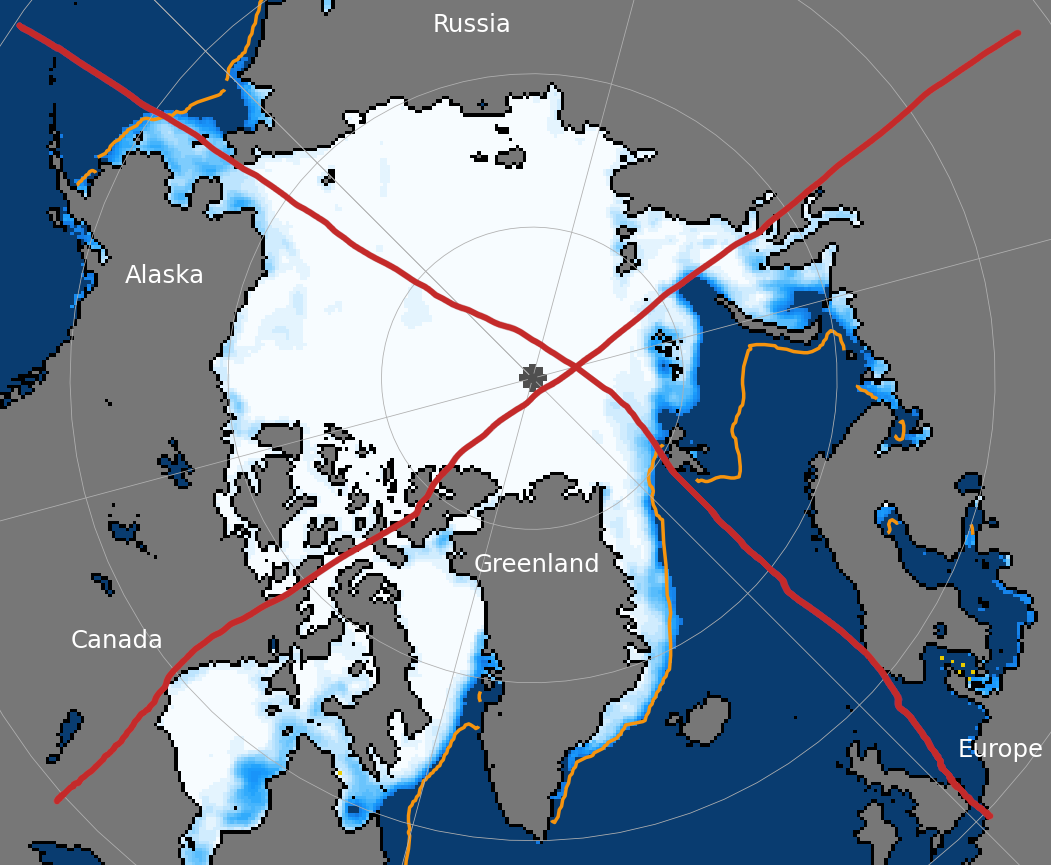
\includegraphics[height=0.8\textheight]{../images/not-sea-ice.png}
\end{center}
\end{frame}


\AtBeginSection[]
{
  \begin{frame}{Outline}
    \tableofcontents[currentsection]
  \end{frame}
}

\section{the basic mathematical model for glaciers}

\basicglaciers{\dots again}

\begin{frame}{modeling simplifications}

\begin{itemize}
\item for simplicity/clarity of the upcoming model, I will \alert{ignore} these aspects of glacier physics in my talk:
    \begin{itemize}
    \item[$\circ$] floating ice
    \item[$\circ$] subglacial hydrology
    \item[$\circ$] ice temperature
    \item[$\circ$] fracture processes (e.g.~calving)
    \item[$\circ$] solid earth deformation
    \end{itemize}

\medskip
\item all are important for doing science!
\item UAF's \href{https://pism.io/}{Parallel Ice Sheet Model (\texttt{pism.io})}, for example, includes these and other processes
\end{itemize}
\end{frame}


\begin{frame}{what is a glacier model?}

\begin{columns}
\begin{column}{0.6\textwidth}
\begin{itemize}
\begin{definition}
a \alert{glacier model} is a \underline{map}

which evolves a glacier in a climate
\end{definition} 
\item at least two inputs:
    \begin{itemize}
    \item[$\circ$] \emph{surface mass balance}
$$\hspace{-7mm} a(t,x,y) = \begin{pmatrix}
\text{snowfall minus} \\
\text{melt \& runoff}
\end{pmatrix}$$

\vspace{-3mm}
        \begin{itemize}
        \item[{\scriptsize $\bullet$}] units of mass flux:\, $\text{kg}\, \text{m}^{-2} \text{s}^{-1}$
        \end{itemize}

    \item[$\circ$] \emph{bed elevation} $b(x,y)$
    \end{itemize}
\item at least two outputs:
    \begin{itemize}
    \item[$\circ$] \emph{upper surface elevation} $s(t,x,y)$
    \item[$\circ$] \emph{ice velocity} $\bu(t,x,y,z)$
    \end{itemize}

\smallskip
\item<2> {\small \underline{map}: \, $\begin{pmatrix} \text{climate \&} \\ \text{topography} \end{pmatrix} \to \begin{pmatrix} \text{geometry} \\ \text{\& velocity} \end{pmatrix}$ }
\end{itemize}
\end{column}
\begin{column}{0.42\textwidth}
\hfill 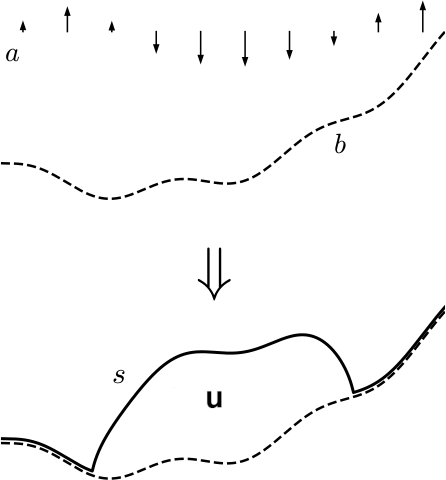
\includegraphics[width=0.9\textwidth]{../images/map-velocity.png}

\vspace{2mm}
\end{column}
\end{columns}
\end{frame}


\begin{frame}{the basic glacier model: notation}

\begin{columns}
\begin{column}{0.55\textwidth}
\begin{itemize}
\item data $a(t,x,y)$, $b(x,y)$ are defined on a \alert{fixed domain}:
	$$t \in [0,T] \quad \text{and} \quad (x,y) \in \Omega \subset \RR^2$$
\item<2-> solution \alert{surface elevation} $s(t,x,y)$ is defined on $[0,T]\times \Omega$
    \begin{itemize}
    \item[$\circ$] also a fixed domain,
    \item[$\circ$] but $s=b$ where there is no ice
    \end{itemize}
\item<3-> $s(t,x,y)$ determines the \alert{icy domain} $\Lambda(t) \subset \RR^3$:
    $$\Lambda(t) = \left\{(x,y,z)\,:\,b(x,y) < z < s(t,x,y)\right\}$$
\item<3-> the solution \alert{velocity} $\bu(t,x,y,z)$ is defined on $\Lambda(t)$

\vspace{-2mm}
\end{itemize}
\end{column}
\begin{column}{0.46\textwidth}
\includegraphics<1>[width=\textwidth]{../images/domain-data.png}

\includegraphics<2>[width=\textwidth]{../images/domain-surface.png}

\includegraphics<3>[width=\textwidth]{../images/domain-velocity.png}
\end{column}
\end{columns}
\end{frame}


\begin{frame}{the basic glacier model: conservation}

\begin{itemize}
\item glacier evolution is merely physics \dots so it \alert{conserves}
    \begin{itemize}
    \item[$\circ$] mass
    \item[$\circ$] momentum
    \item[$\circ$] energy \hfill $\leftarrow$ \emph{ignored for simplicity in this talk}
    \end{itemize}

\medskip
\item<2> conservation of mass happens
    \begin{itemize}
    \item[$\circ$] within the icy domain $\Lambda(t) \subset \RR^3$:
\begin{align*}
\text{\alert{incompressibility}}&& \Div \bu &= 0 \qquad \text{in } \Lambda(t) \\
    \intertext{\item[$\circ$] on the surfaces $\Gamma_s(t), \Gamma_b(t) \subset \partial \Lambda(t)$:}
\text{\alert{surface kinematic equation (SKE)}}&& \frac{\partial s}{\partial t} - \bu|_s \cdot \bn_s &= a \qquad \text{on } \Gamma_s(t) \\
\text{\alert{non-penetration}}&&     \bu|_b \cdot \bn_b &= 0 \qquad \text{on } \Gamma_b(t)
\end{align*}

        \begin{itemize}
        \item[$\vartriangleright$] $\Gamma_s(t)$ is upper surface of the ice
        \item[$\vartriangleright$] $\Gamma_b(t)$ is base of the ice
        \item[$\vartriangleright$] $\bn_s = \left<-\grad s,1\right>$ is upward surface normal
        \end{itemize}
    \end{itemize}

\end{itemize}
\end{frame}


\begin{frame}{the free boundary problem for a fluid layer}

\begin{itemize}
\item glacier evolution is a \alert{free-boundary} problem
\item specifically, the surface kinematic equation (SKE)
  $$\frac{\partial s}{\partial t} - \bu|_s \cdot \bn_s = a$$
applies \emph{only} on the ice upper surface $\Gamma_s(t)$
\item in the remainder of the (fixed) domain $\Omega\subset \RR^2$, \alert{complementarity} holds:
  $$s=b \quad \text{and} \quad a \le 0$$

\bigskip
\item {\footnotesize for more on this perspective see Bueler (2021), \emph{Conservation laws for free-boundary fluid layers}, SIAM J.~Appl.~Math}
\end{itemize}
\end{frame}


\begin{frame}{the basic glacier model strong form: \, NCP coupled to Stokes}

\begin{itemize}
\item \only<1>{\alert{nonlinear complementarity problem} (NCP)} \only<2>{nonlinear complementarity problem (NCP) coupled to \alert{Stokes}}:
\begin{align*}
s - b &\ge 0 && \text{on $\Omega \subset \RR^2$} \\
\frac{\partial s}{\partial t} - \bu|_s \cdot \bn_s - a &\ge 0 && \text{''} \\
(s - b) \left(\frac{\partial s}{\partial t} - \bu|_s \cdot \bn_s - a\right) &= 0 && \text{''} \\
\onslide<2->{- \nabla \cdot \left(2 \nu(D\bu)\, D\bu\right) + \nabla p - \rhoi \mathbf{g} &= \bzero && \text{in $\Lambda(t) \subset \RR^3$} \\
\nabla \cdot \bu &= 0 && \text{''} \\
\btau_b - \bbf(\bu|_b) &= \bzero && \text{on $\Gamma_b(t)$} \\
\bu|_b \cdot \bn_b &= 0 && \text{''} \\
\left(2 \nu(D\bu) D\bu - pI\right) \bn_s &= \bzero && \text{on $\Gamma_s(t)$}}
\end{align*}

    \begin{itemize}
    \item[$\circ$] note: $\bu|_s=0$ where no ice
    \item<2->[$\circ$] viscosity by Glen law: \, $2\nu(D\bu) = \Gamma |D\bu|^{\pp-2}$, \,$p \approx 4$
    \end{itemize}
\end{itemize}
\end{frame}


\begin{frame}{the basic glacier model is a DAE system}

\begin{itemize}
\item for this slide, forget complementarity and boundary conditions to get simplified model ``SKE coupled to Stokes'':
\begin{align*}
\frac{\partial s}{\partial t} - \bu|_s \cdot \bn_s - a &= 0 \\
- \nabla \cdot \left(2 \nu(D\bu)\, D\bu\right) + \nabla p - \rhoi \mathbf{g} &= \bzero \\
\nabla \cdot \bu &= 0
\end{align*}

\item only the first of these 5 equations has a time derivative
    \begin{itemize}
    \item[$\circ$] recall: ice is very viscous and incompressible
    \end{itemize}
\item<2> this time-dependent problem is a \alert{differential algebraic equation} (DAE), an extremely stiff system:
\begin{align*}
\dot x &= f(x,y) \\
     0 &= g(x,y)
\end{align*}

    \begin{itemize}
    \item<2>[$\circ$] in $\infty$ dimensions, of course,
    \item<2> and also subject to complementarity
    \end{itemize}
\end{itemize}
\end{frame}


\begin{frame}{the basic glacier model: current research}

\begin{itemize}
\item to the best of my knowledge, \emph{no} current research groups are studying well-posedness or regularity for this basic model
    \begin{itemize}
    \item[$\circ$] though most researchers would agree NCP-coupled-to-Stokes is indeed the intended model!
    \end{itemize}

\medskip
\item<2> progress has been made on well-posedness of the lubrication approximation of the basic model, the so-called \alert{shallow ice approximation}:
    \begin{itemize}
    \item[$\circ$] 1D well-posedness on flat bed (Calvo et al 2002)
    \item[$\circ$] 2D steady-state existence on general beds (Jouvet \& Bueler 2012)
    \item[$\circ$] 2D well-posedness on flat bed (Piersanti \& Temam 2022)
    \end{itemize}
\end{itemize}
\end{frame}


\begin{frame}{the basic glacier model: current numerical \emph{thinking}}

\begin{itemize}
\item numerical glacier and ice sheet modelers tend to think of the Stokes problem separately from surface evolution
    \begin{itemize}
    \item[$\circ$] \emph{time-splitting} or \emph{explicit time-stepping} is often taken for granted
    \end{itemize}

\medskip
\item \dots and ice sheet geometry evolution is often addressed with minimal awareness of complementarity

\medskip
\item<2> the NCP-coupled-to-Stokes basic model is \emph{not yet} in common use for high-resolution, long-duration ice sheet simulations
    \begin{itemize}
    \item[$\circ$] because it is too slow
    \item[$\circ$] \alert{can we make it fast enough to use?} \hfill \begin{minipage}{0.3\textwidth}{\footnotesize \color{FireBrick}{$\leftarrow$ \emph{what I am working on}}} \end{minipage}
    \end{itemize}
\end{itemize}
\end{frame}


\section{numerics: time-stepping}

\begin{frame}{the mass-continuity equation view}

\begin{itemize}
\item ``thickness transport form'' helps for evolution or stability questions
\item define:
\begin{align*}
H(t,x,y) &=s-b && \text{ice thickness} \\
\bU(t,x,y) &= \frac{1}{H} \int_b^s \bu \,dz && \begin{matrix} \text{vertically-averaged} \\ \hspace{-1.8mm} \text{horizontal velocity} \end{matrix}
\end{align*}

    \begin{itemize}
    \item[$\circ$] note $s$ and $H$ are equivalent variables for modeling ice geometry
    \end{itemize}
\item the \alert{mass continuity equation} for thickness, an apparent \alert{advection equation}, follows from the SKE and incompressibility:
   $$\frac{\partial H}{\partial t} + \nabla \cdot \left(\bU H\right) = a$$

\smallskip
\item<2> \emph{question:} is this really an advection equation?
\item<2>[] \emph{answer:} not really \dots ice flows (mostly) downhill so
  $$\bU \sim - \grad s \sim - \grad H$$
\item<2> in any case, the NCP-coupled-to-Stokes system \emph{has no characteristic curves}
\end{itemize}
\end{frame}


\begin{frame}{mass continuity equation: advection or diffusion?}

\begin{align*}
\text{advective schema:} && \frac{\partial H}{\partial t} + \nabla \cdot \left(\bU H\right) &= a \\
\text{diffusion schema:} && \frac{\partial H}{\partial t} - \nabla \cdot \left(D \grad s\right) &= a
\end{align*}
\begin{itemize}
\item both forms are nonlinear: \, $\bU=\bU(H,\grad s), \, D=D(H,\grad s)$
\item the glacier modeling literature is confusing!
\item the diffusion schema is literal in the shallow ice approximation
    \begin{itemize}
    \item[$\circ$] more on this momentarily
    \end{itemize}
\item regardless of your schema preference, the fact that ice flows downhill has \emph{time-stepping stability} consequences!
\item \dots so let us recall some traditional numerical analysis
\end{itemize}
\end{frame}


\begin{frame}{traditional PDE time-stepping}

{\footnotesize
\begin{align*}
\text{advective schema:} && \frac{\partial H}{\partial t} + \nabla \cdot \left(\bU H\right) &= a \\
\text{diffusion schema:} && \frac{\partial H}{\partial t} - \nabla \cdot \left(D \grad s\right) &= a
\end{align*}
}

\begin{minipage}[t][60cm][t]{\textwidth}
\begin{itemize}
\only<1>{
\item \alert{explicit} time stepping is common for \alert{advections}
\item for example, forward Euler using spacing $h$ and time step $\Delta t$:
	$$\frac{H_j^{\ell+1} - H_j^\ell}{\Delta t} + \frac{\bq_{j+1/2}^\ell - \bq_{j-1/2}^\ell}{h} = a_j^\ell$$

    \begin{itemize}
    \item[$\circ$] need good approximations of flux $\bq=\bU H$: upwinding, Lax-Wendroff, streamline diffusion, flux-limiters, \dots
    \item[$\circ$] conditionally stable, with CFL maximum time step
        $$\Delta t \le \frac{h}{\max |\bU|} = O(h)$$
    \end{itemize}
}
\only<2>{
\item \alert{explicit} time stepping for \alert{diffusions} is best avoided
\item for example, forward Euler:
	$$\frac{H_j^{\ell+1} - H_j^\ell}{\Delta t} - \frac{D_{j+\frac{1}{2}} (s_{j+1}^{\ell} + s_{j}^{\ell}) - D_{j-\frac{1}{2}} (s_{j}^{\ell} + s_{j-1}^{\ell})}{h^2} = a_j^\ell$$

    \begin{itemize}
    \item[$\circ$] conditionally stable, with maximum time step
        $$\Delta t \le \frac{h^2}{\max D} = O(h^2)$$
    \end{itemize}
}
\only<3>{
\item \alert{implicit} time stepping for \alert{diffusions} is often recommended
\item for example, backward Euler:
	$$\frac{H_j^{\ell+1} - H_j^\ell}{\Delta t} - \frac{D_{j+\frac{1}{2}} (s_{j+1}^{\ell+1} + s_{j}^{\ell+1}) - D_{j-\frac{1}{2}} (s_{j}^{\ell+1} + s_{j-1}^{\ell+1})}{h^2} = a_j^\ell$$

    \begin{itemize}
    \item[$\circ$] unconditionally stable, but must solve equations at each step
    \item[$\circ$] further implicit schemes: Crank-Nicolson, BDF, \dots
    \end{itemize}
}
\end{itemize}
\end{minipage}
\end{frame}


\begin{frame}{time-stepping in current ice sheet models}

\begin{itemize}
\item current-technology, large-scale numerical models, including \href{https://www.pism.io/}{PISM}, use explicit time stepping
    \begin{itemize}
    \item[$\circ$] this is embarrassing: the mathematical problem is a DAE
    \end{itemize}
\item many researchers ``believe'' the advection schema
    \begin{itemize}
    \item[$\circ$] time step is supposed to be determined by CFL using the coupled solution velocity $\bU$
    \end{itemize}
\item the accuracy/performance/usability consequences of the suppressed DAE/diffusive character are hard to sweep under the rug
\item the whole situation is a cry for mathematical clarity!
\end{itemize}
\end{frame}


\begin{frame}{time-stepping in \emph{future} ice sheet models}

\begin{itemize}
\item \alert{implicit time-stepping} is appropriate for DAE problems
\item future models will solve a sequence of NCP-coupled-to-Stokes free-boundary problems at each time step
\end{itemize}
\end{frame}


\section{numerics: Stokes models}

\begin{frame}{shallow ice approximation \quad $\leftarrow$ \emph{not Stokes}}

\begin{itemize}
\item the simplest of glacier flow approximations is the ``lubrication'' approximation: \alert{shallow ice approximation} (SIA)
\item SIA version of the NCP:
{\small
  $$s - b \ge 0, \quad \frac{\partial s}{\partial t} + {\color{FireBrick} \Phi(s)} - a \ge 0, \quad (s - b) \left(\frac{\partial s}{\partial t} + {\color{FireBrick} \Phi(s)} - a\right) = 0$$
}
the surface motion contribution ${\color{FireBrick} \Phi(s) = - \bu|_s \cdot \bn_s}$ has a formula:
  $${\color{FireBrick} \Phi(s)} = - \frac{\gamma}{\pp} (s-b)^{\pp} |\grad s|^{\pp} - \grad \cdot\left(\frac{\gamma}{\pp+1} (s-b)^{\pp+1} |\grad s|^{\pp-2} \grad s\right)$$

\vspace{-2mm}
    \begin{itemize}
    \item[$\circ$] constants $\pp = \nn+1$ and $\gamma > 0$ relate to ice deformation
    \end{itemize}

\medskip
\item ${\color{FireBrick} \Phi(s)}$ is a \alert{doubly-nonlinear differential operator}
    \begin{itemize}
    \item[$\circ$] porous medium and $\pp$-Laplacian type simultaneously
    \item[$\circ$] but \emph{local} in surface and bed topography, which Stokes is not
    \item[$\circ$] well-posedness holds for the weak form $=$ \alert{variational inequality} (Calvo et al 2002, Jouvet \& Bueler 2012, Piersanti \& Temam 2022)
    \end{itemize}
\end{itemize}
\end{frame}


\begin{frame}{nonlocality}

\begin{itemize}
\item however, from now on, let us avoid shallowness approximations
\item the basic glacier model (NCP coupled to Stokes) problem has a \alert{non-local} surface velocity function ${\color{FireBrick} \Phi(s) = - \bu|_s \cdot \bn_s}$
{\small
\begin{equation*}
s - b \ge 0, \quad \frac{\partial s}{\partial t} + {\color{FireBrick} \Phi(s)} - a \ge 0, \quad (s - b) \left(\frac{\partial s}{\partial t} + {\color{FireBrick} \Phi(s)} - a\right) = 0
\end{equation*}
}
\item the Stokes velocity solution responds to a surface perturbation by up- and down-stream changes, for several ice thicknesses, \onslide<2>{while the SIA velocity responds only underneath the surface perturbation}
\end{itemize}

\begin{center}
\includegraphics<1>[width=0.6\textwidth]{../images/stokes-greens-arndt.png}
\includegraphics<2>[width=0.6\textwidth]{../images/sia-greens-arndt.png}
\end{center}
\end{frame}


\begin{frame}{the Stokes problem for ice}

\begin{itemize}
\item a non-shallow model solves a Stokes problem at each step:
\begin{align*}
- \nabla \cdot \left(2 \nu(D\bu)\, D\bu\right) + \nabla p - \rhoi \mathbf{g} &= \bzero && \text{in $\Lambda \subset \RR^3$} \\
\nabla \cdot \bu &= 0 && \text{''} \\
\btau_b - \bbf(\bu|_b) &= \bzero && \text{on $\Gamma_b$} \\
\bu|_b \cdot \bn_b &= 0 && \text{''} \\
\left(2 \nu(D\bu) D\bu - pI\right) \bn_s &= \bzero && \text{on $\Gamma_s$}
\end{align*}
\item this is the \alert{stress balance} (conservation of momentum) problem which determines velocity $\bu$ and pressure $p$
\item<2> how fast is the numerical solution process?
    \begin{itemize}
    \item[$\circ$] how do solution algorithms \alert{scale} with increasing spatial resolution?
    \end{itemize}
\end{itemize}
\end{frame}


\begin{frame}{one slide course: numerical PDE solver algorithmic scaling}

\begin{itemize}
\item consider the Poisson equation:
    $$-\grad^2 u = f \,\text{ in $\Omega$}, \qquad u=0 \,\text{ on $\partial\Omega$}$$
\item discretization generates a linear system $A\,\bu = \bb$ with $\bu\in\RR^m$
\item the number of unknowns is the data size $m$:
    \begin{itemize}
    \item[$\circ$] $m$ = \#(nodes in the mesh)
    \item[$\circ$] $m$ scales with mesh cell diameter: \quad $m \sim h^{-2}$ \quad in 2D
    \end{itemize}
\item \alert{complexity} or \alert{algorithmic scaling} of flops, as $m\to\infty$, depends on solver algorithm:
    \begin{itemize}
    \item[$\circ$] $O(m^3)$ for direct linear algebra, ignoring matrix structure
    \item[$\circ$] $\approx O(m^2)$ for sparsity-exploiting direct linear algebra
    \item[$\circ$] $O(m^1)$, \alert{optimal}, for \alert{multigrid} solvers
    \end{itemize}
\end{itemize}

\medskip
\begin{center}
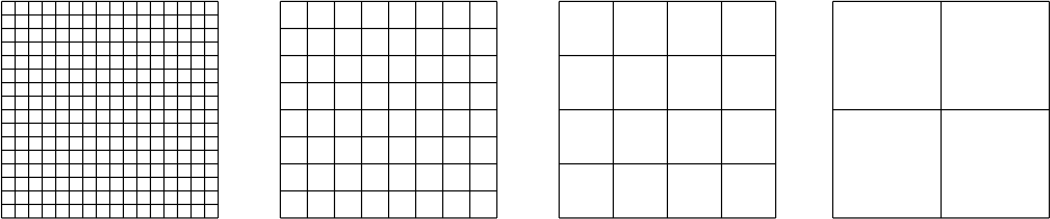
\includegraphics[width=0.5\textwidth]{../images/multigrid-grids.png}
\end{center}
\end{frame}


\begin{frame}{ice sheet models: stress-balance solver complexity}

\begin{itemize}
\item Stokes: \quad $m$ = \#(velocity and pressure unknowns)
\item model the scaling as $O(m^{1+\alpha})$, with $\alpha=0$ optimal
\item \alert{near-optimal solvers} already exist: \hfill $\leftarrow$ \emph{good news!}
    \begin{itemize}
    \item[$\circ$] $\alpha=0.08$ for Isaac et al.~(2015) Stokes solver
        \begin{itemize}
        \item[$\vartriangleright$] unstructured quadrilateral/tetrahedral mesh, $Q_k\times Q_{k-2}$ stable elements, Schur-preconditioned Newton-Krylov, ice-column-oriented algebraic multigrid (AMG) preconditioner for $(\bu,\bu)$ block
        \end{itemize}

\begin{center}
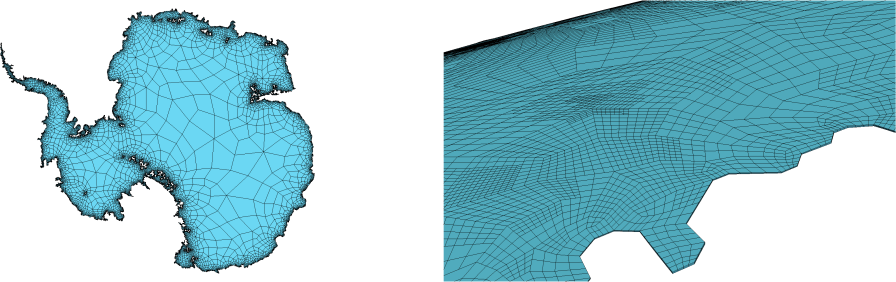
\includegraphics[width=0.6\textwidth]{../images/isaac-antarctica.png}
\end{center}
    \item[$\circ$] $\alpha=0.05$ for Tuminaro et al~(2016) 1st-order (shallow) AMG solver
    \item[$\circ$] similar for Brown et al~(2013) 1st-order (shallow) GMG solver
    \end{itemize}
\item \emph{but} this is for Stokes solvers \alert{de-coupled} from the surface-evolution NCP
\end{itemize}
\end{frame}



\section{numerics: comparative performance analysis}

\begin{frame}{ice sheet models: the analysis set-up}

\begin{itemize}
\item ice sheets are thin layers, thus ice sheet models often have $O(1)$ mesh points in the vertical direction
    \begin{itemize}
    \item[$\circ$] e.g.~Issac et al (2015) Stokes solver
    \item[$\circ$] I am ignoring refinement in the vertical
    \end{itemize}

\medskip
\item data size: \quad {\small $m$ = \#(surface elevation \& velocity \& pressure unknowns)}
\item assume domain $\Omega \subset \RR^2$ with width $L$ and cell diameter $h$:
  $$m \sim \frac{L^2}{h^2} \hspace{20mm}$$

\vspace{-14mm}
\hfill
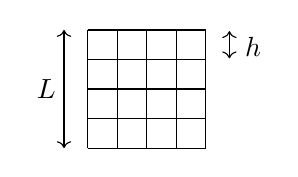
\begin{tikzpicture}[scale=1.5]
  \pgfmathsetmacro\fourth{1.0/4.0}
  \draw[xstep=\fourth,ystep=\fourth,black,thin] (0.0,0.0) grid (1.0,1.0);
  \draw[<->] (-0.2,0.0) -- (-0.2,1.0);
  \draw[<->] (1.2,0.76) -- (1.2,0.99);
  \node at (-0.35,0.5) {$L$};
  \node at (1.4,0.86) {$h$};
\end{tikzpicture}

\vspace{-2mm}
\item recall explicit time-stepping stability:
{\footnotesize
\begin{align*}
\text{advective} && \frac{\partial H}{\partial t} + \nabla \cdot \left(\bU H\right) &= a & &\implies & \Delta t &\le \frac{h}{U} \\
\text{diffusion} && \frac{\partial H}{\partial t} - \nabla \cdot \left(D \grad s\right) &= a & &\implies & \Delta t &\le \frac{h^2}{D}
\end{align*}
}

\item recall stress-balance solver complexity: \quad $O(m^{1+\alpha})$
\end{itemize}
\end{frame}


\begin{frame}{ice sheet models: the performance question}

\begin{itemize}
\item glaciologists want to run time-stepping high-resolution simulations of ice sheets over e.g.~$10^5$ year ice age cycles

\bigskip
\item proposed metric: \quad \alert{flops per model year}

\bigskip
\item the question:

\bigskip
\begin{center}
\begin{minipage}{0.82\textwidth}
how does this metric \alert{scale} in the \alert{high spatial resolution limit} $h\to 0$, equivalently $m\to \infty$?
\end{minipage}
\end{center}

\bigskip
\item the goal is optimality: \hspace{20mm} $\text{flops} \sim O(h^{-2}) = O(m^1)$
\end{itemize}
\end{frame}


\begin{frame}{ice sheet models: explicit time-stepping performance}

\begin{tabular}{llll}
\emph{time-stepping} &  & \emph{flops per model year} \\ \hline
\\
explicit & SIA    & $\oo{\frac{D\, L^2}{h^{\,4}}} = \oo{\frac{D}{L^2} m^{\,2}}$ \\
\\
explicit ({\footnotesize \emph{advective}}) & Stokes \phantom{xxxx} & $\oo{\frac{U \,L^{2+2\alpha}}{h^{\,3+2\alpha}}} = \oo{\frac{U}{L} m^{1.5+\alpha}}$ \\
\\
\phantom{explicit} ({\footnotesize \emph{diffusive}})  & Stokes & $\oo{\frac{D\, L^{2+2\alpha}}{h^{\,4+2\alpha}}} = \oo{\frac{D}{L^2} m^{\,2+\alpha}}$
\end{tabular}


\vspace{10mm}
\begin{itemize}
\item we \emph{want} optimality: \quad $O(m^1)$ flops per model year
\item explicit time-stepping implies \alert{too many stress-balance solves}
    \begin{itemize}
    \item[$\circ$] while the Stokes (stress-balance) scaling exponent $\alpha$ is important, even Stokes solver optimality ($\alpha=0$) cannot yield optimality
    \end{itemize}
\end{itemize}
\end{frame}


\begin{frame}{implicit time-stepping for ice sheet models}

\begin{itemize}
\item let us try \alert{implicit time-stepping}, for its unconditional stability
\item each step is now a \alert{free-boundary NCP-coupled-to-Stokes problem}
\item let us parameterize cost of these solves as $O(m^{1+\beta})$
\item we still need $q$ model updates per year to integrate climate influences, and track evolution for the simulation purpose
\end{itemize}
\end{frame}


\begin{frame}{ice sheet model performance table (Bueler, 2022)}

\begin{tabular}{llll}
\emph{time-stepping} &  & \emph{flops per model year} \\ \hline
\\
explicit & SIA    & $\oo{\frac{D\, L^2}{h^{\,4}}} = \oo{\frac{D}{L^2} m^{\,2}}$ \\
\\
explicit ({\footnotesize \emph{advective}}) & Stokes \phantom{xxxx} & $\oo{\frac{U \,L^{2+2\alpha}}{h^{\,3+2\alpha}}} = \oo{\frac{U}{L} m^{1.5+\alpha}}$ \\
\\
\phantom{explicit} ({\footnotesize \emph{diffusive}})  & Stokes & $\oo{\frac{D\, L^{2+2\alpha}}{h^{\,4+2\alpha}}} = \oo{\frac{D}{L^2} m^{\,2+\alpha}}$ \\
\\
implicit & & $\oo{\frac{q\, L^{2+2\beta}}{h^{\,2+2\beta}}} = \oo{q\, m^{1+\beta}}$
\end{tabular}

\bigskip
\begin{itemize}
\item new goal: use implicit time-stepping \emph{and}~build a $\beta \approx 0$ NCP-coupled-to-Stokes solver for problem at each time step
\end{itemize}
\end{frame}


\begin{frame}{existing implicit models?}

\begin{itemize}
\item no convincing NCP-coupled-to-Stokes (free-boundary) solvers exist yet
    \begin{itemize}
    \item[$\circ$] however, Wirbel \& Jarosch~(2020) is an important beginning
    \end{itemize}
\item the Bueler (2016) implicit and NCP SIA solver scales badly: $\beta=0.8$
\end{itemize}
\end{frame}


\section{a multilevel approach}

\begin{frame}{multilevel NCP-coupled-to-Stokes solvers}

\begin{itemize}
\item FIXME
\item direct attack on the problem seems to require a \alert{multilevel} solver for \alert{variational inequalities} (VIs)
\item but in the non-local residual case this seems not to exist
    \begin{itemize}
    \item[$\circ$] the \alert{smoother} must reduce a residual formed from surface-motion term $\Phi(s) = - \bu|_s\cdot \bn_s$ (from a scalable Stokes solver)
    \end{itemize}
\item near-optimal multilevel solvers exist for simpler VI problems
\end{itemize}
\end{frame}


\section{conclusion}

\begin{frame}{\alert{summary}}

\begin{itemize}
\item glacier simulations are both \alert{important to humanity} and a rich \alert{source of interesting mathematics}
   \begin{itemize}
   \item[$\circ$] predict sea level rise!
   \end{itemize}
\item<2-> ice sheet models solve a multi-scale, irregular-data problem with hard-to-observe boundary conditions
   \begin{itemize}
   \item[$\circ$] there are \alert{no easy or magic techniques} for performance
   \end{itemize}
\item<3-> current-technology ice sheet models mostly use \alert{explicit} time stepping, \alert{non-optimal} stress-balance solvers, and \alert{shallow} assumptions
   \begin{itemize}
   \item[$\circ$] progress is being made in all of these areas, e.g.~scalable Stokes solvers (Isaac et al.~2015)
   \end{itemize}
\item<4> scalable solvers for implicit-step, NCP-coupled-to-Stokes models require \alert{multilevel solvers for non-local variational inequalities}
   \begin{itemize}
   \item[$\circ$] is this the preferred numerical design for the basic glacier model?
   \end{itemize}
\end{itemize}
\end{frame}


\begin{frame}{references (partial list)}

{\scriptsize
\begin{itemize}
\item E.~Bueler (2016). \emph{Stable finite volume element schemes for the shallow-ice approximation}, J.~Glaciol.~62 (232), 230--242, \href{https://doi.org/10.1017/jog.2015.3}{10.1017/jog.2015.3}
%\item E.~Bueler (2021). \emph{Conservation laws for free-boundary fluid layers}, SIAM J.~Appl.~Math.~81 (5), 2007--2032, \href{https://doi.org/10.1137/20M135217X}{10.1137/20M135217X}
\item E.~Bueler (2022). \emph{Performance analysis of high-resolution ice-sheet simulations}, J.~Glaciol., \href{https://doi.org/10.1017/jog.2022.113}{10.1017/jog.2022.113}
\item E.~Bueler \& P.~Farrell (in preparation). \emph{A full approximation storage multilevel method for nonlinear variational inequalities}
\item N.~Calvo, J.~D\'iaz, J.~Durany, E.~Schiavi, \& C.~V\'azquez (2002). \emph{On a doubly-nonlinear parabolic obstacle problem modelling ice sheet dynamics}, SIAM J.~Appl.~Math., 63(2), 683--707 \href{https://doi.org/10.1137/S0036139901385345}{10.1137/S0036139901385345}
\item T.~Isaac, G.~Stadler, \& O.~Ghattas (2015). \emph{Solution of nonlinear Stokes equations discretized by high-order finite elements on nonconforming and anisotropic meshes, with application to ice sheet dynamics}, SIAM J.~Sci.~Comput.~37 (6), B804--B833, \href{https://doi.org/10.1137/140974407}{10.1137/140974407}
\item G.~Jouvet \& E.~Bueler (2012). \emph{Steady, shallow ice sheets as obstacle problems: well-posedness and finite element approximation}, SIAM J.~Appl.~Math.~72 (4), 1292--1314, \href{https://doi.org/10.1137/110856654}{10.1137/110856654}
\item P.~Piersanti \& R.~Temam (2022). \emph{On the dynamics of grounded shallow ice
sheets: modeling and analysis}, Adv.~Nonlinear Analysis 12, \href{https://doi.org/10.1515/anona-2022-0280}{10.1515/anona-2022-0280}
\item A.~Wirbel \& A.~Jarosch (2020). \emph{Inequality-constrained free-surface evolution in a full Stokes ice flow model (evolve\_glacier v1.1)}, Geosci.~Model Dev.~13 (12), 6425--6445, \href{https://doi.org/10.5194/gmd-13-6425-2020}{10.5194/gmd-13-6425-2020}
\end{itemize}
}
\end{frame}

\end{document}
